\documentclass[a4paper,11pt]{report}
\usepackage[T1]{fontenc}
\usepackage[utf8]{inputenc}
\usepackage[polish]{babel}
\usepackage{lmodern}
\usepackage{graphicx}
\usepackage{geometry}

\title{Różne przypadki złożoności obliczeniowej algorytmu Quicksort}
\author{Monika Litwin 200586}
\begin{document}
\maketitle

\begin{figure}
  \begin{center}
  \textbf{Trochę teorii}
\\
\begin{flushleft}\underline{Przypadek optymistyczny}\end{flushleft}
Teoretycznie takowy występuje, gdy sortowany jest już uporządkowany zbiór \\(z niewielką ilością elementów nie na swoich miejscach). \\Wtedy złożoność wynosi \emph{O(nlogn)}

\begin{flushleft}\underline{Przypadek typowy}\end{flushleft}
Zbiór poddany algorytmowi sortowania posiada losowo rozłożone elementy.\\ Złożoność wynosi \emph{O(nlogn)}

\begin{flushleft}\underline{Przypadek pesymistyczny}\end{flushleft}
Występuje dla zbiorów o elementach posortowanych odwrotnie.\\ Złożoność wynosi \emph{O($ n^{2}$)}

    \label{fig:}
  \end{center}
\end{figure}

\begin{figure}
  \begin{center}
	\textbf{Sortowanie zbioru odwrotnie posortowanych elementów}
\\ Poniżej zamieszczony jest wykres pomiarów czasu dla algorytmu, któremu podano wcześniej posortowany w odwrotnej kolejności wektor. Testy wykonano dla przypadku, gdy pivot wybierany jest w sposób losowy lub zawsze jest elementem środkowym.
Czas sortowania jest krótszy, gdy pivot jest losowy.

    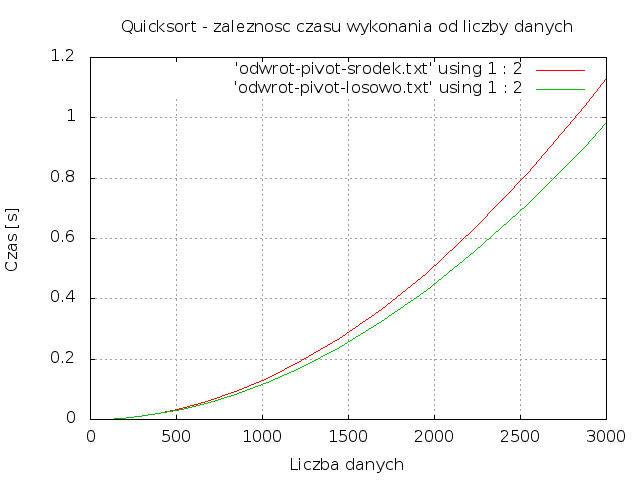
\includegraphics[scale=0.5]{./odwrotnie.png}
    \label{fig:}
  \end{center}
\end{figure}

\begin{figure}
  \begin{center}
  \textbf{Sortowanie zbioru posortowanych elementów}
\\W kolejnym teście porównuję wpływ wyboru pivota na czas sortowania dla przetwarzania posortowanego już wektora. Tutaj również algorytm wykonywał się szybciej, gdy pivot wybierany był losowo.
\\
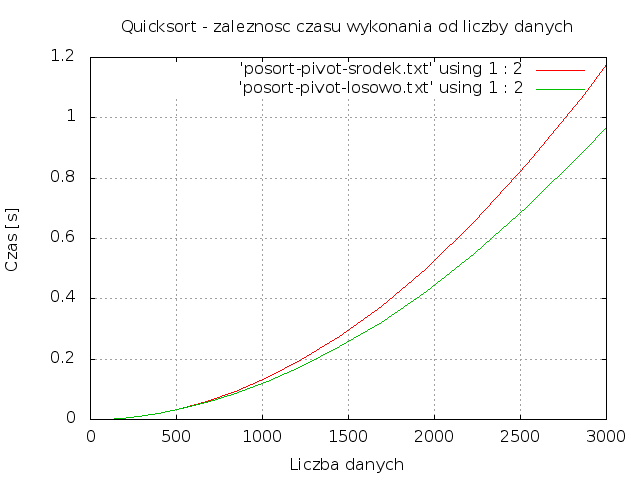
\includegraphics[scale=0.5]{./posortowane.png}
  \end{center}
\end{figure}

\begin{figure}
  \begin{center}
  \textbf{Sortowanie zbioru nieposortowanych elementów}
\\
Gdy sortujemy zbiór nieuporządkowanych elementów sytuacja jest identyczna, jak w poprzednich dwóch przypadkach - algorytm wykonuje się szybciej, kiedy pivot wybierany jest losowo.

    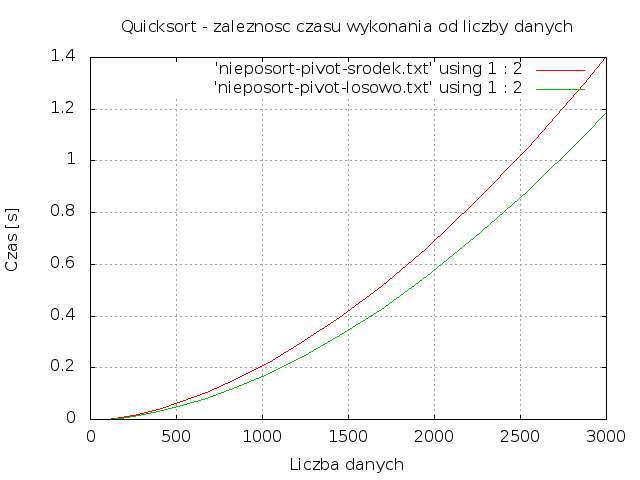
\includegraphics[scale=0.5]{./nieposotrowane.png}
    \label{fig:}
  \end{center}
\end{figure}

\begin{figure}
  \begin{center}
  \textbf{Sortowanie elementów z losowo wybieranym pivotem}
  \\Tutaj obserwujemy szybkość wykonania algorytmy Quicksort z losowym pivotem dla zbiorów: nieposortowanego, posortowanego oraz posortowanego odwrotnie. Zdecydowanie najwięcej czasu potrzeba było na posortowanie elementów wcześniej nieposortowanych. Pozostałe przypadki są bardzo zbliżone czasowo do siebie.
  \\
  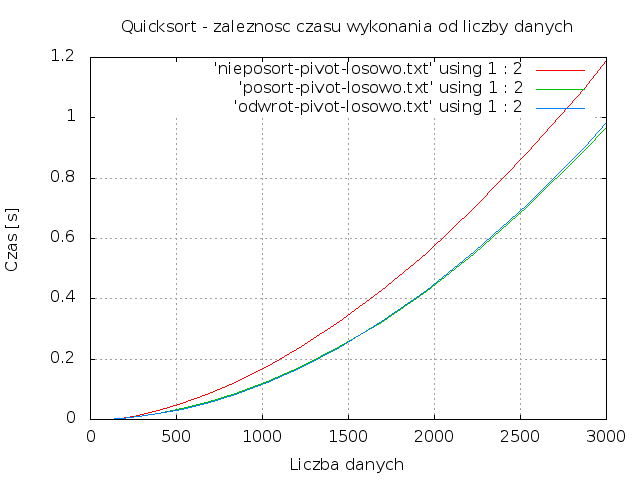
\includegraphics[scale=0.5]{./pivot-losowo.png}
    \label{fig:}
  \end{center}
\end{figure}

\begin{figure}
  \begin{center}
  \textbf{Sortowanie elementów z pivotem po środku}
  \\Na poniższym wykresie obserwujemy sytuację niemal identyczną, jak na poprzednim. Najdłużej sortuje się zbiór nieposortowany, pozostałe - podobnie czasowo.
  \\
  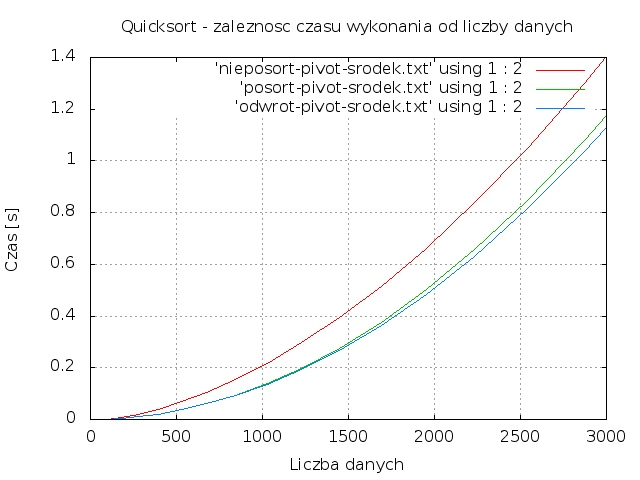
\includegraphics[scale=0.5]{./pivot-srodek.png}
    \label{fig:}
  \end{center}
\end{figure}

\begin{figure}
  \begin{center}
  \textbf{Wnioski}
  \\
Można zaobserwować, że losowe dobieranie pivota faktycznie usprawniło działanie algorytmu. Widać wyraźną różnicę na wykresach obrazujących czas sortowania (pierwsze trzy). 
\\
Jeśli chodzi o porównanie przedstawionej teorii z praktycznymi wynikami, to nie zaobserwowałam przypadku pesymistycznego. Miał on wystąpić przy sortowaniu odwrotnie posortowanych elementów. W rzeczywistości czas sortowania takiego zbioru jest bardzo zbliżony do sortowania elementów posortowanych we właściwym porządku. Zarówno, gdy pivot jest dobierany losowo, jak i wtedy gdy zawsze jest elementem środkowym. Wyraźnie za to odbiega przypadek sortowania nieuporządkowanego \\zbioru - czas jest dłuższy.



    \label{fig:}
  \end{center}
\end{figure}

\end{document}
